%% PNAStwoS.tex
%% Sample file to use for PNAS articles prepared in LaTeX
%% For two column PNAS articles
%% Version1: Apr 15, 2008
%% Version2: Oct 04, 2013



%% BASIC CLASS FILE
\documentclass{pnastwo}






% And another fix.  PNAS class loses the label of floats unless they       
% were defined with the [h] option (so not really floats at all).  It      
% all comes down to wrong scope in the following routine which pushes      
% out the floats onto the page.  This is the fixed version:        
\makeatletter                                  
\def\DonormalEndcol{%                              
%% top float ==>                               
\ifx\toporbotfloat\xtopfloat%                          
%% figure ==>                                  
  \ifcaptypefig%                               
  \expandafter\gdef\csname topfloat\the\figandtabnumber\endcsname{%    
  \vbox{\vskip\PushOneColTopFig%                       
  \unvbox\csname figandtabbox\the\loopnum\endcsname%               
  \vskip\abovefigcaptionskip%                          
  \csname caption\the\loopnum\endcsname%                   
  \csname letteredcaption\the\loopnum\endcsname%               
  \csname continuedcaption\the\loopnum\endcsname%              
  \csname letteredcontcaption\the\loopnum\endcsname            
  \ifredefining%                               
  \csname label\the\loopnum\endcsname%                     
  \expandafter\gdef\csname topfloat\the\loopnum\endcsname{}\fi}%       
  \vskip\intextfloatskip%%                         
  \vskip-4pt %% probably an artifact of topskip??              
}%                                     
\else%                                     
%% plate ==>                                   
  \ifcaptypeplate%                             
  \expandafter\gdef\csname topfloat\the\figandtabnumber\endcsname{%    
  \vbox{\vskip\PushOneColTopFig%                       
  \unvbox\csname figandtabbox\the\loopnum\endcsname            
  \vskip\abovefigcaptionskip                           
  \csname caption\the\loopnum\endcsname                    
  \csname letteredcaption\the\loopnum\endcsname                
  \csname continuedcaption\the\loopnum\endcsname               
  \csname letteredcontcaption\the\loopnum\endcsname            
  \ifredefining                                
  \csname label\the\loopnum\endcsname                      
  \expandafter\gdef\csname topfloat\the\loopnum\endcsname{}\fi}        
  \vskip\intextfloatskip %%                            
  \vskip-4pt %% probably an artifact of topskip??              
}%                                     
\else% table ==>                               
 \expandafter\gdef\csname topfloat\the\figandtabnumber\endcsname{%     
 \vbox{\vskip\PushOneColTopTab %%                      
 \csname caption\the\loopnum\endcsname                     
  \csname letteredcaption\the\loopnum\endcsname                
  \csname continuedcaption\the\loopnum\endcsname               
  \csname letteredcontcaption\the\loopnum\endcsname            
  \vskip\captionskip                               
  \unvbox\csname figandtabbox\the\loopnum\endcsname            
\ifredefining                                  
\csname label\the\loopnum\endcsname                    
\expandafter\gdef\csname topfloat\the\loopnum\endcsname{}\fi           
}\vskip\intextfloatskip %% why don't we need this?             
\vskip-10pt}                                   
\fi\fi%                                    
%                                      
\else% bottom float                            
%                                      
\ifcaptypefig                                  
\expandafter\gdef\csname botfloat\the\figandtabnumber\endcsname{%      
\vskip\intextfloatskip                             
\vbox{\unvbox\csname figandtabbox\the\loopnum\endcsname            
\vskip\abovefigcaptionskip                         
  \csname caption\the\loopnum\endcsname                    
  \csname letteredcaption\the\loopnum\endcsname%               
  \csname continuedcaption\the\loopnum\endcsname%              
  \csname letteredcontcaption\the\loopnum\endcsname%               
\vskip\PushOneColBotFig%%                          
\ifredefining%                                 
\csname label\the\loopnum\endcsname                    
\expandafter\gdef\csname botfloat\the\loopnum\endcsname{}\fi}}%        
\else                                      
\ifcaptypeplate                                
\expandafter\gdef\csname botfloat\the\figandtabnumber\endcsname{%      
\vskip\intextfloatskip                             
\vbox{\unvbox\csname figandtabbox\the\loopnum\endcsname            
\vskip\abovefigcaptionskip                         
  \csname caption\the\loopnum\endcsname                    
  \csname letteredcaption\the\loopnum\endcsname%               
  \csname continuedcaption\the\loopnum\endcsname%              
  \csname letteredcontcaption\the\loopnum\endcsname%               
\vskip\PushOneColBotFig%%                          
\ifredefining%                                 
\csname label\the\loopnum\endcsname                    
\expandafter\gdef\csname botfloat\the\loopnum\endcsname{}\fi}}%        
  \else% TABLE                                 
\expandafter\gdef\csname botfloat\the\figandtabnumber\endcsname{%      
  \vskip\intextfloatskip                           
\vbox{\csname caption\the\loopnum\endcsname                
  \csname letteredcaption\the\loopnum\endcsname                
  \csname continuedcaption\the\loopnum\endcsname               
  \csname letteredcontcaption\the\loopnum\endcsname%               
  \vskip.5\intextfloatskip                         
  \unvbox\csname figandtabbox\the\loopnum\endcsname%               
\vskip\PushOneColBotTab                            
\ifredefining%                                 
\csname label\the\loopnum\endcsname                    
\expandafter\gdef\csname botfloat\the\loopnum\endcsname{}\fi}}%        
\fi\fi\fi}                                 
\makeatother  


%Fix wierd behavior which prevents table captions from appearing for
% tables in the body of the article
\makeatletter
\long\def\@makecaption#1#2{%
\ifx\@captype\table
\let\currtabcaption\relax
\gdef\currtabcaption{
\tabnumfont\relax #1. \tabtextfont\relax#2\par
\vskip\belowcaptionskip 
}
\else
 \vskip\abovecaptionskip
  \sbox\@tempboxa{\fignumfont#1.\figtextfont\hskip.5em\relax #2}%
  \ifdim \wd\@tempboxa >\hsize
\fignumfont\relax #1.\figtextfont\hskip.5em\relax#2\par
  \else
    \global \@minipagefalse
    \hb@xt@\hsize{\hfil\box\@tempboxa\hfil}%
  \fi
\fi
}
\makeatother


\usepackage{adjustbox}
\usepackage{array}

% \newcolumntype{R}[2]{%
%     >{\adjustbox{angle=#1,lap=\width-(#2)}\bgroup}%
%     l%
%     <{\egroup}%
% }
\newcolumntype{R}[2]{%
    >{\adjustbox{angle=#1,lap=\width-(#2)}\bgroup}%
    l%
    <{\egroup}%
}
\newcommand*\rot{\multicolumn{1}{R{75}{0em}}}% no optional argument here, please!


\setlength{\footskip}{.5in}
\usepackage{algorithm2e}
%% ADDITIONAL OPTIONAL STYLE FILES Font specification
\usepackage{natbib}
\usepackage{bm}% bold math
%\newcommand{\bm}[1]{\boldsymbol{#1}} %makes bold math symbols easier
\newcommand{\R}{\textsf{R}\space} %R in textsf font
\newcommand{\X}{\bm{\mathcal{X}}} %shorthand for iid
\renewcommand{\P}{\mathcal{P}}
\newcommand{\bt}{\pmb{\theta}}
\newcommand{\bl}{\pmb{\lambda}}
\newcommand{\bL}{\pmb{\Lambda}}
%\newcommand{\bG}{\pmb{\Gamma}}
\newcommand{\bh}{\pmb{\text{h}}}
\newcommand{\h}{\pmb{\text{h}}}
\usepackage{amsmath,amssymb,amsthm}
\def\citeapos#1{\citeauthor{#1}'s (\citeyear{#1})}
\DeclareMathOperator*{\argmax}{arg\,max}

%\graphicspath{{/Users/matthewjdenny/Dropbox/PINLab/Projects/Denny_Working_Directory/2011_Analysis_Output}}

%\usepackage{pnastwoF}
\usepackage{hyperref,booktabs,tabularx,float}


%% OPTIONAL MACRO DEFINITIONS
\def\s{\sigma}


\begin{document}

\title{Reading between the Emails: Gendered Patterns of Communication in Local Government}

\author{
Matthew Denny\affil{1}{Penn State University},
James ben-Aaron\affil{2}{University of Massachusetts Amherst},
Hanna Wallach\affil{2}{}\affil{3}{Microsoft Research NYC},
\and Bruce Desmarais\affil{1}{}
}

\contributor{\vspace{-.25cm}}


\maketitle

\begin{article}
\begin{abstract}
	
{In this paper, we study the role of gender in local government
organizations. We analyze email data from seventeen county
governments in North Carolina to understand the relationship
between a department manager's gender and the emails they send
and receive. First, we use descriptive statistics to identify
aggregate gender-homophilous and gender-heterophilous patterns
from the numbers of emails sent and received by all department
managers. In contrast to previous research, we find no strong
evidence of either gender homophily or heterophily. To
investigate this finding, we therefore analyze
department-to-department communication patterns. Here, we do find
evidence of gender bias, with some departments exhibiting gender
homophily and others exhibiting heterophily. Finally, to
determine the extent to which these patterns are driven by
communication content, we use a recently developed latent
variable model to identify topic-specific communication
subnetworks for each county. We find differing degrees of gender
homophily and heterophily for different topics of
communication. From a policy perspective, these findings suggest
that a gender-equitable working environment cannot be created by
hiring decisions alone, as gender bias in communication still
exists independent of the positions held by men and women.
}
\end{abstract} 

%\keywords{gender | public records | email | network}

%\abbreviations{SAM, self-assembled monolayer; OTS, octadecyltrichlorosilane}

\section{Gender in Organizations}
Researchers have observed and documented gender bias in both the
public and private sectors. Women receive lower pay, hold less
prestigious positions, have reduced opportunities for advancement, and
are excluded from the organizational locus of control \citep{Brass1985, Bielby1986a, Ibarra1992, Albrecht2003, Duncan2004}. As a result,
organizations that aspire to a just, efficient, and sustainable
professional culture strive to provide men and women with equal
treatment in the workplace \citep{Ely2000}. In practice, however, these organizations
have historically found it hard to understand the micro-level causes
of gender bias. The limited availability of primary source data has lead most previous research to rely on observational, ethnographic, or self-reported data \citep[e.g.,][]{Castilla2005, Adams2007, Elsesser2011}. This makes it challenging to understanding these causes because such data can be biased, and are often limited in scope. 
	
However, with the increasing use of electronic communication, and the rise of transparency initiatives within government, scholars are now able to use public records requests to gather primary source email communication data. Using public records requests as a method for data collection also provides a major benefit of making the data collection process replicable. Therefore, we choose to study the relationship between a department manager's gender, and the emails they send and receive, in a sample of local governments. To do this, we collect and analyze a large scale email data set from a sample of seventeen county governments in North Carolina. 

We begin by examining the aggregate patterns of email communication among department managers in these counties by gender, and the gender breakdown of managers for each department. Then we analyze interdepartmental email flows by gender of the email sender and its recipients. Finally, we apply a statistical model for communication network data to infer the topic-conditional structure of manager-to-manager email communication in these county governments. Our results indicate that while aggregate patterns of communication among department managers do not display significant gender bias, the topics of communication, and positions held by men and women differ significantly.


\section{Data}

The data used in this study were collected in 2013 via a series of public records requests made to all one hundred North Carolina county governments. We selected North Carolina for our data collection efforts because the state public records laws cover email data, and prevent counties from charging unreasonable fees for providing data. Twenty-three counties complied with our request, of which seventeen provided data was useable for our research\footnote{Some counties provided too little data (i.e. 30 emails for the entire county), or provided data in paper form, which was not amenable to our analyses.}. Our records request to each county included all emails sent and received by all department managers (e.g. Health, Finance, Elections) over a three-month period in 2013\footnote{Requests to each county specified a random starting month for the request, between January and October, 2103.}. 

We received approximately 500,000 emails from the seventeen county governments which provided useable data, of which approximately 17,000 were sent between county department managers, which we focus on in the analyses presented here. Figure \ref{fig:nc map} highlights the counties which responded to our requests for data. We also collected detailed metadata on the department and gender of the 362 department managers in our sample. We display some basic descriptive statistics for each county in table \ref{tab:county aggregate stats}. Approximately 40\% of department managers in our sample are women, although there is significant variation in the proportion of female department managers across counties. It is important to note that the counties in our sample are statistically indistinguishable from the rest of the counties in North Carolina on a number of demographic dimensions including population, per-capita income, and percent of the population that is white.


	\begin{figure}
		\centering
	\caption{\label{fig:nc map} North Carolina map with counties who provided useable data highlighted.}	
	\centering
	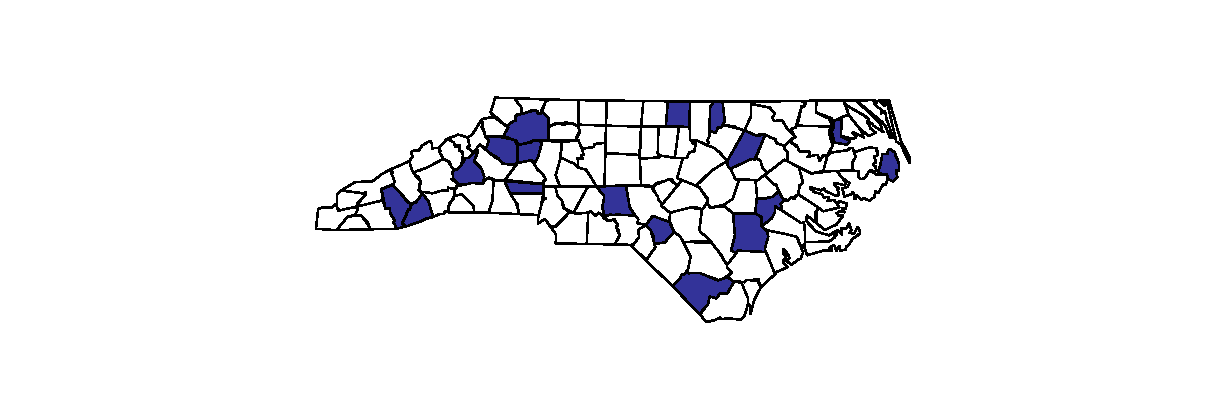
\includegraphics[width = 0.48\textwidth]{images/County_Map.pdf}
	\end{figure}
	
	\begin{table}
	\centering
		\begin{tabular}{lrrrr}
		  \toprule
		  % add an extra line
		  & \multicolumn{2}{c}{\textbf{Manager Gender}} & \\
		  \cmidrule{2-3}
		 \textbf{County} & \textbf{Male} & \textbf{Female} & \textbf{Emails Sent}  \\
		  \midrule
		Alexander & 12 & 9 & 907   \\
		Caldwell & 12 & 8 & 121     \\
		Chowan & 12 & 11 & 2,027   \\
		Columbus & 14 & 10 & 920   \\
		Dare & 15 & 12 & 2,247    \\
		Duplin & 13 & 14 & 1,914    \\
		Hoke & 13 & 11 & 1,106  \\
		Jackson & 18 & 6 & 1,499    \\
		Lenoir & 15 & 5 & 560  \\
		Lincoln & 15 & 7 & 573   \\
		McDowell & 12 & 5 & 326   \\
		Montgomery & 8 & 10 & 680   \\
		Nash & 11 & 8 & 1,147  \\
		Person & 12 & 9 & 1,491   \\
		Transylvania & 16 & 4 & 1,857  \\
		Vance & 10 & 8 & 185   \\
		Wilkes & 15 & 2 & 303   \\
		   \midrule
		   \textbf{Totals:} & 362 & 139 & 17,863 \\
		   \bottomrule
		\end{tabular}
		\caption{\label{tab:county aggregate stats}Breakdown of department managers by gender, and the total number of emails sent by department managers, for each county in our sample.}
	\end{table}



\section{Descriptive Analysis}

We begin our analysis of the relationship between a department manager's gender and the emails they send and receive, by looking for differences in the propensity for department managers to send emails to other managers of the same gender (\emph{gender-homophilous} communication), and managers of the opposite gender (\emph{gender-heterophilous} communication). Table \ref{tab:email agg stats} provides some basic descriptive statistics including the average number emails sent and received by male and female department managers in our sample. On average, male and female department managers send and receive a comparable number of emails, and emails sent by male and female department managers have a similar number of recipients. Therefore, if we observe gender differences in email communication, they are unlikely to be driven by some innate difference in the propensity for male and female department managers to send or receive emails. 
	
	\setlength{\tabcolsep}{2pt}
	\begin{table}
	\centering
		\begin{tabular}{m{2.1in}rrr}
		\toprule
		& \multicolumn{2}{c}{\textbf{Manager Gender}} \\
		\cmidrule{2-3}
	& \textbf{Male} & \textbf{Female}  \\
		 \midrule
		 % Proportion of Managers in Sample & 61.6\%& 38.4\% \\
		 % \midrule
		 Average \# of emails sent & 48.3 & 51 \\
		 Average \# of recipients per email sent & 1.45 & 1.43 \\
		 \midrule
		 Average \# of emails received & 70.8 & 71.6 \\
		\bottomrule
		\end{tabular}
		\caption{\label{tab:email agg stats}Email statistics by manager
gender.\\}
	\end{table}
	\setlength{\tabcolsep}{6pt}

To test whether the gender of an email sender is related to the gender of its recipients, in aggregate, we construct a contingency table of email sending and receiving by gender (see table \ref{tab:gender email agg stats}). We then perform a $\chi^2$ test for independence between the rows and columns. The $\chi^2$ test statistic we obtain indicates that the gender of an email sender and its recipients is not independent $(\chi^2 = 92.9, p < 0.001)$. However, inspection of the contingency table indicates that the test statistic is actually driven by mild gender heterophily in communication. Furthermore, the gender differences we observe are substantively quite small, as both male and female department managers send emails to recipients of each gender in rough proportion to their overall representation in the sample (60\% to men, 40\% to women).  
	
	% make this a contingency table and do a chi squared test
	\begin{table}
	\centering
		\begin{tabular}{rlrr|r}
		\toprule
		 && \multicolumn{3}{c}{\textbf{Recipient}} \\
		\cmidrule{3-5}
	& & \textbf{Male} & \textbf{Female} & \textbf{Total}  \\
		 \midrule
		$|$& \textbf{Male} & 7,299 & 6,286 & 13,585 \\
	\textbf{Sender}	$|$& \textbf{Female} & 5,325 & 3,510 & 8,835 \\
	\cmidrule{2-5}
		 $|$& \textbf{Total} & 12,624 & 9,796 & \\
		\bottomrule
		\end{tabular}
		\caption{\label{tab:gender email agg stats}Each cell records the number of times a department manager of gender X was included as a recipient of an email sent by a department manager of gender Y. Statistics provided are calculated for all counties combined. Note that each email may have more than one recipient.}
	\end{table}
	
This result contradicts what we know about gender-driven interaction in the workplace, and is possibly a result of the vast majority of e-mails being substantively uninteresting (e.g. meeting reminders sent automatically from a manager's Microsoft Outlook account). Therefore, we need to partition e-mails according to content in order to observe substantively interesting patterns. Our data allow us to use the department of each manager as a rough proxy for the content of their email communication. We begin by looking for aggregate differences in the gender breakdown of department managers for each department, across our sample (see table \ref{tab:gender position}). Departments were hand coded into one of twenty-five different categories based on the title given in the county directory, to group departments that perform a similar function. Note that not all departments are represented in each county.

	% latex table generated in R 3.2.2 by xtable 1.7-4 package
	% Sat Sep 19 21:03:09 2015
	\setlength{\tabcolsep}{4pt}
	\begin{table}
	\centering
	 \caption{\label{tab:gender position} Number of male and female managers for each department.\\ }        \bigskip
	\begin{tabular}{rrrrrrrrrrrrrrr}
		\toprule
	 & \rot{\textbf{Emergency}} & \rot{\textbf{Health}} & \rot{\textbf{IT}} & \rot{\textbf{Manager}} & \rot{\textbf{HR}} & \rot{\textbf{Library}} & \rot{\textbf{Plan/Dev}} & \rot{\textbf{Deeds}} & \rot{\textbf{Parks/Rec}} & \rot{\textbf{Finance}} & \rot{\textbf{Soc/Serv}} & \rot{\textbf{Veterans}} & \rot{\textbf{Util/Waste}}  \\ 
	  \midrule
	  \textbf{Male} & 15 & 5 & 11 & 15 & 3 & 3 & 11 & 6 & 9 & 5 & 8 & 5 & 11  \\ 
	\textbf{Female} & 2 & 11 & 2 & 2 & 12 & 8 & 3 & 9 & 5 & 12 & 8 & 7 & 1  \\ 
	  
	   \bottomrule
	   & \rot{\textbf{Elections}} & \rot{\textbf{Sheriff}} & \rot{\textbf{Info}} & \rot{\textbf{Tax}} & \rot{\textbf{Inspections}} & \rot{\textbf{Animal}} & \rot{\textbf{Maintenance}} & \rot{\textbf{Seniors}} & \rot{\textbf{Transport}} & \rot{\textbf{Environment}} & \rot{\textbf{Misc}} & \rot{\textbf{Extension}} \\
	   \midrule
	   \textbf{Male} &  2 & 16 & 2 & 10 & 11 & 9 & 5 & 2 & 6 & 7 & 5 & 8 \\
	   \textbf{Female} & 11 & 1 & 5 & 5 & 3 & 3 & 0 & 6 & 1 & 4 & 1 & 5 \\
	   \bottomrule
	\end{tabular}
	
	\end{table}
	\setlength{\tabcolsep}{6pt}
	
	
We can see that some departments are mostly managed by men: the county manager (the supervisor of all other department managers), the sheriff, and the emergency manager, for example. Other departments  are mostly managed by women: the HR, finance, and health departments, for example. A a $\chi^2$ test for the independence of department and gender confirms our qualitative finding that there is a strong bias in which departments tend to be managed by women $(\chi^2 = 130.8, p < 0.001)$. This result indicates a bias in the gender breakdown of department managers for each department, across our sample, but cannot tell us about differences in email communication by men and women who manage the same department. To answer this question, we need to know whether the gender of an email sender and the gender of its recipients is independent of the their respective departments. 
	
	\begin{figure*}
	\centering
	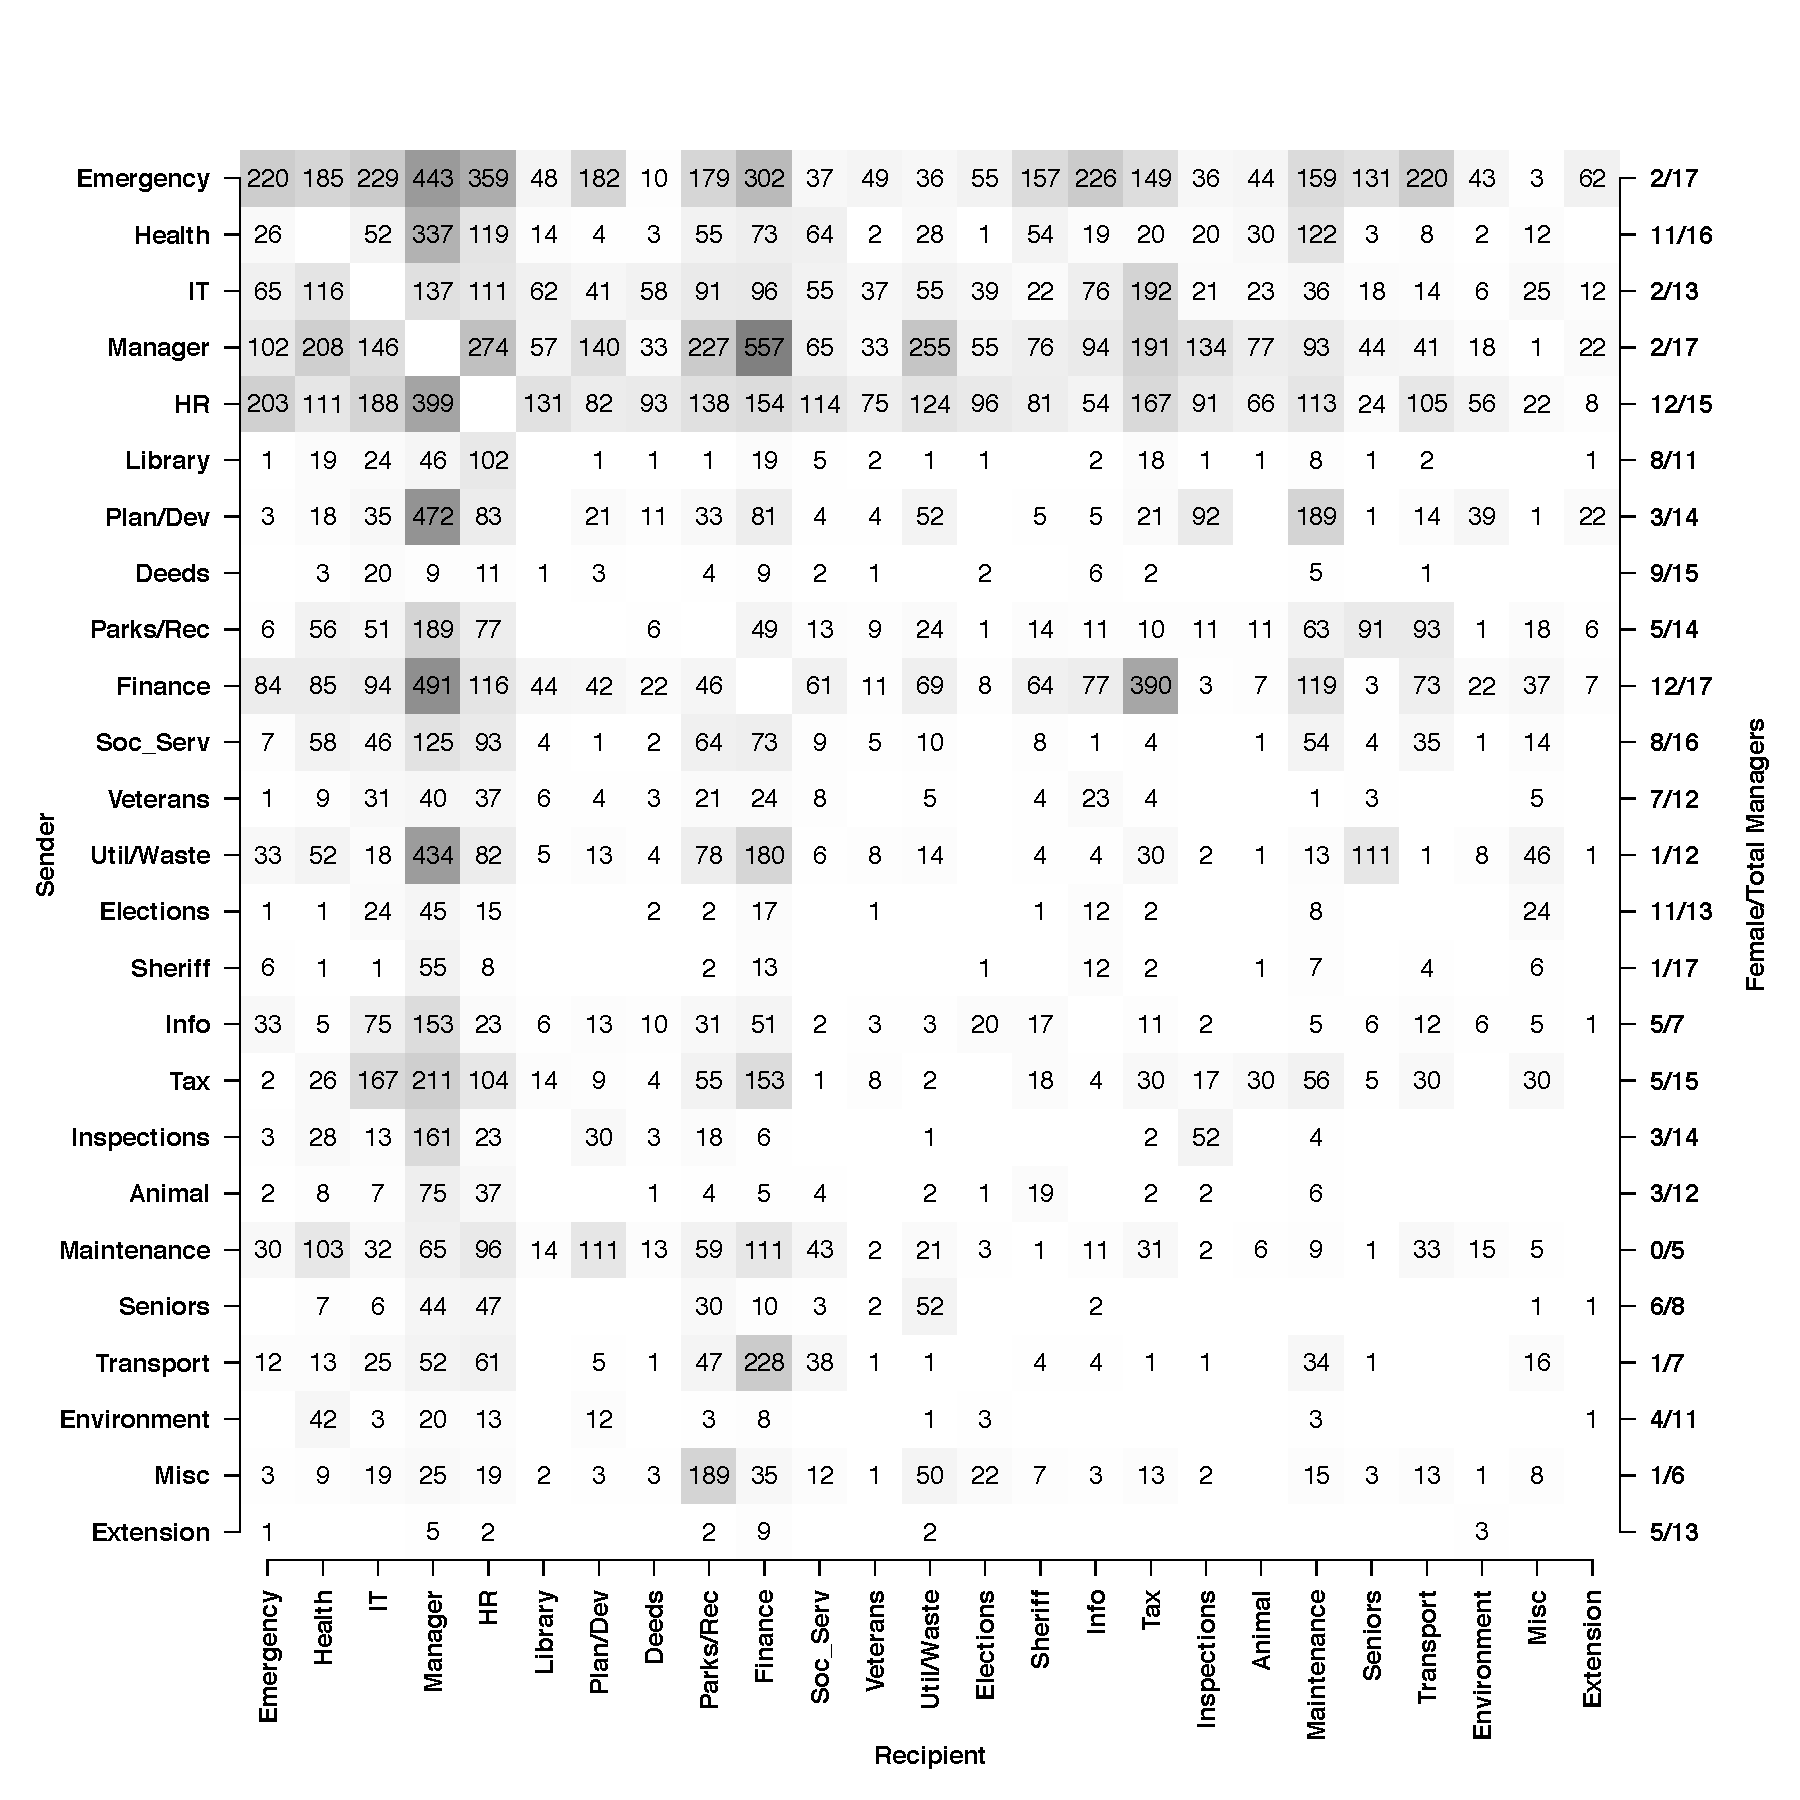
\includegraphics[width = 0.8\textwidth]{images/Aggregate_Email_Flows.pdf}
	\caption{\label{fig:heatmaps}Heat map depicting the total number of emails sent from the managers of each department to the managers of each other department, aggregated across counties. The right-hand y-axis displays the number of counties that had that department, and the number of those managers who were women. Departments are ordered by the total number emails their managers sent.}
	\end{figure*}

	
	
Table \ref{fig:heatmaps} displays the aggregate number of times each department manager was a recipient of an email sent by a manager of each other department. We see pronounced differences in email sending an receiving by department, but cannot graphically disentangle the role of gender. 
%To test for the independence of the gender of an email sender and the gender of its recipients, from the departments they direct, 
Next, we construct a contingency table of department dyad-types (where each ``dyad-type'' is a unique combination of sender and recipient department, eg. finance $\longrightarrow$ HR) against gender dyad-types (where each ``dyad-type'' is a unique combination of sender and recipient gender, eg. male $\longrightarrow$ female).  We then perform a $\chi^2$ test on this contingency table, which indicates that the gender of an email sender and its recipients is not independent of their respective departments ($\chi^2 = 37,404, p < 0.001$).
	
	
This dyadic $\chi^2$ test tells us that there is an association between gender mixing patterns and department mixing patterns. Indeed, when we construct similar contingency tables for each department, we find that email senders in utilities and waste management departments exhibit gender-homophilous behavior ($\chi^2 = 10.49, p < 0.001$), senders in the tax department exhibit gender-heterophilous behavior ($\chi^2 = 4.54, p < 0.034$), and senders in the IT department seem unbiased ($\chi^2 = 1.23, p > 0.27$). However, we can't say from these results that the form of gender bias depends upon the domain of interaction since factors other than content are likely to vary with department labels, including the county in which the manager is working, the experience of the manager, and the manager's status in the organizational hierarchy. To disentangle these effects, we need explicitly model the topical content of emails. To do this, we extend a recently introduced joint model for communication topical content and network structure \citep{Krafft2012}, and apply it to our email data.
	


\section{A Model of Email Content}
Here we provide a brief overview of our extension to the topic-partitioned
multinetwork embedding (TPME) model \citep{Krafft2012}. In particular, we illustrate how this model lets us make inferences about the gender-specific patterns of communication in organizations, and how these patterns change with the topics of communication. Our model follows Krafft et al. \citep{Krafft2012} by integrating the latent space network model (LSM) \citep{Hoff2002a} with latent Dirichlet allocation (LDA) \cite{Blei2003} to jointly model the content and structure of an email network. This model is designed to be applied to email data where we observe each message sender and its recipients, as well as the email content (the words). 

At a high level, our model assumes the following generative process for a message sent across the email network. First, we sample the content of the message following the generative process for LDA. Then, for a given message sender, we draw whether each other actor in the network is a recipient of that message following the LSM. However, different topics are associated with different latent spaces, so how likely each actor is to be a recipient of a particular message is dependent on the topical content of that message. We review this process in greater detail below.  

%  \begin{figure}
% \caption{\label{fig:splitting} Different patterns of communication across different domains.}
% \centering
% 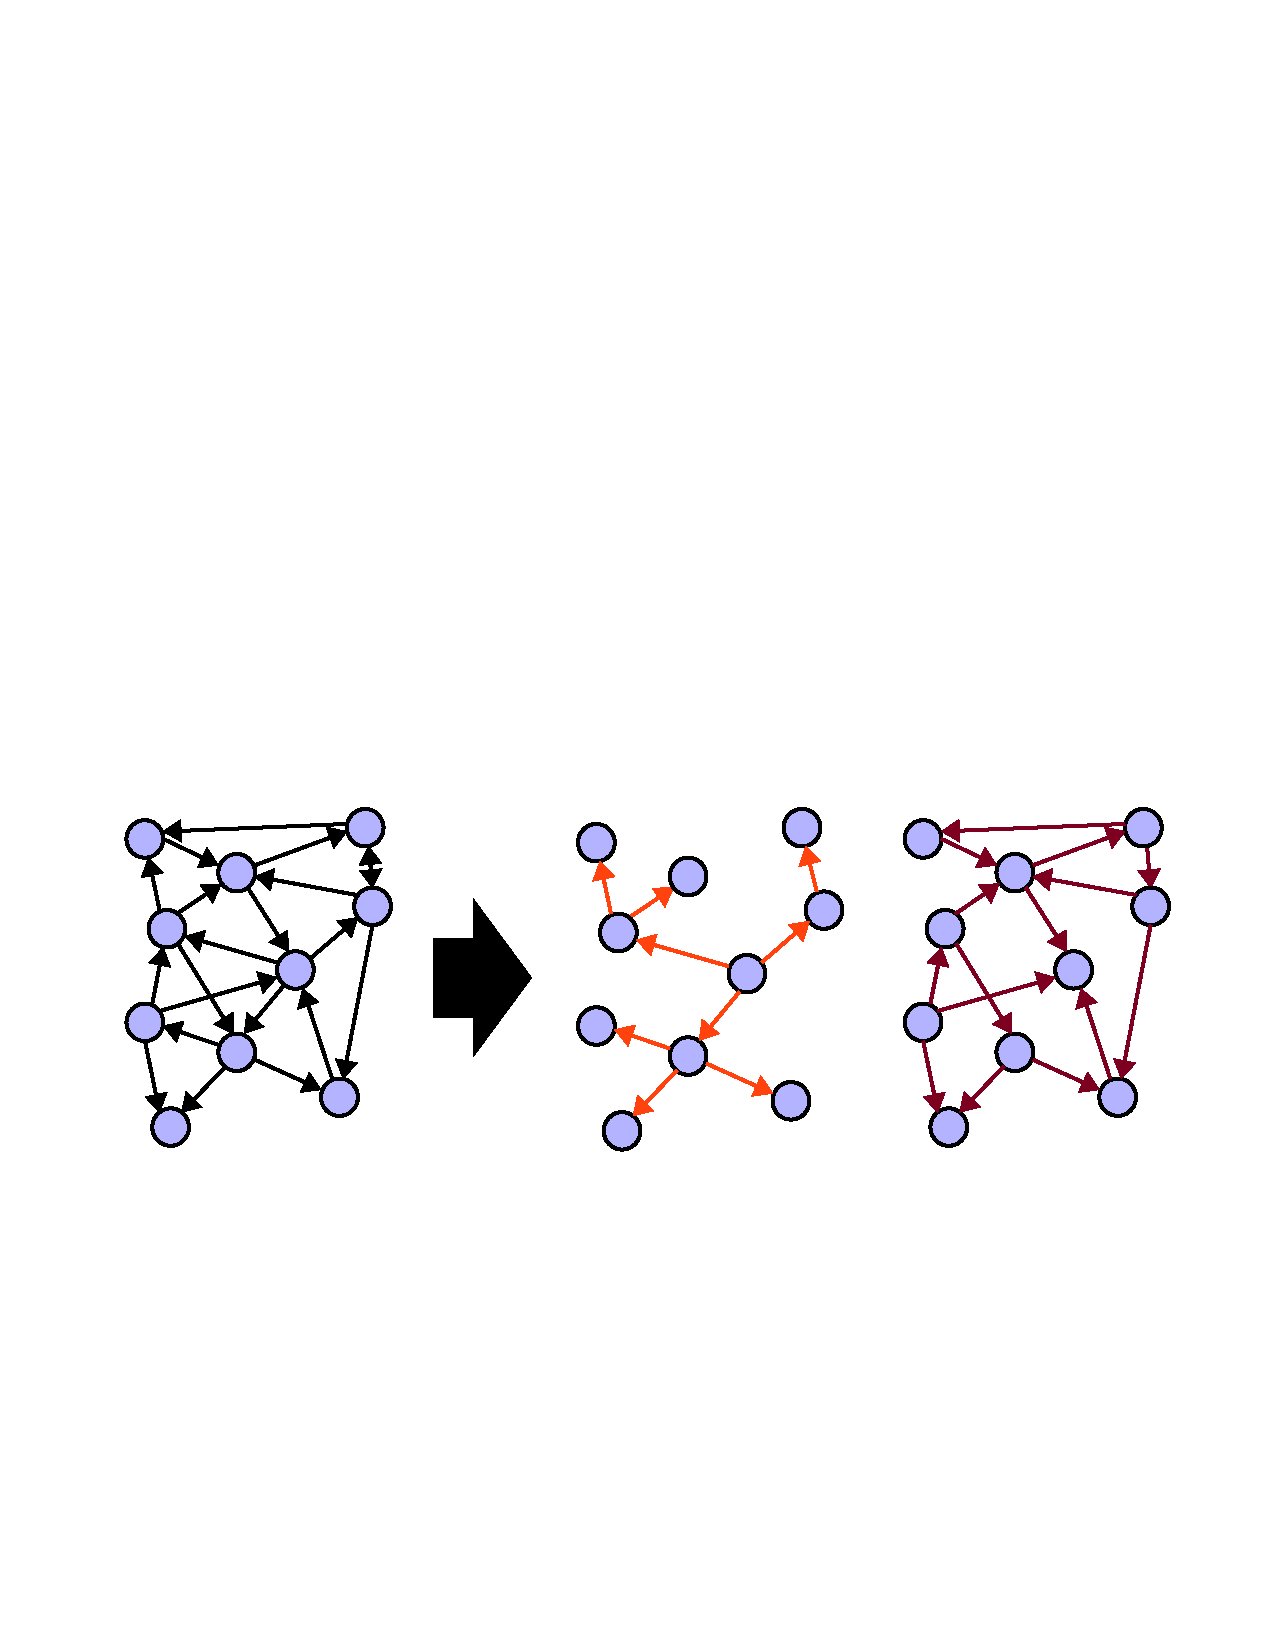
\includegraphics[width = 0.48\textwidth]{images/Structure_Matters_Full.pdf}
% \end{figure}

The message content is assumed to be generated via LDA. Under this model, we assume that all unique words in our vocabulary are associated to varying degrees with each of $T$ latent \emph{topics}. Each topic is then a distribution over unique words (or \emph{word types}), $\boldsymbol{\phi}^{(t)}$. For example \emph{doctor}, \emph{virus}, and \emph{medicine} might all have high probability in a topic about hospitals, while \emph{cat} and \emph{music} might have low probability in that topic. We further assume that each topic distribution is drawn from a Dirichlet prior: 
\begin{equation}
	\boldsymbol{\phi}^{(t)} \sim \text{Dirichlet}(\beta,\boldsymbol{n}) \text{ for } t = \{1, ..., T\}
\end{equation}
where the base measure $\boldsymbol{n}$ is the mean of the distribution, and the concentration parameter $\beta$ controls how concentrated typical draws are around that mean. 
%For example, \emph{patient} might generally have a higher probability than most word types in a corpus of documents about healthcare, and this could be represe.   

To generate each of the $D$ documents (messages) in our corpus, we first draw a document-specific distribution over topics:
\begin{equation}
	\boldsymbol{\theta}^{(d)} \sim \text{Dirichlet}(\alpha,\boldsymbol{m}) \text{ for } d = \{1,...,D\}
\end{equation}
%Here, the concentration parameter $\alpha$ controls how specific the distributions over topics in the documents generated are, and $\boldsymbol{m}$ controls the bias in how likely certain topics are to appear. 
Once we have drawn our document-specific distribution over topics we can then generate each of $N$ tokens (words) in the document via a two step process. First we draw the latent topic assignment for that token from the document specific distribution over topics.
\begin{equation}
	z_n^{(d)} \sim \boldsymbol{\theta}^{(d)} \text{ for } n = \{1,...,N\}
\end{equation}
 Then we draw the word type of that token from the topic specific distribution over word types.
 \begin{equation}
 	w_n^{(d)} \sim \boldsymbol{\phi}^{(z_n^{(d)})} \text{ for } n = \{1,...,N\}
 \end{equation}
We proceed in this manner for all tokens in all documents. 


In our extension of TPME, we further assume each topic is uniquely associated with one of $C$ clusters, drawn from a discrete uniform distribution.
\begin{equation}
	C_t \sim \text{U}(1,...,C) \text{ for } t = \{1, ..., T\}
\end{equation}
The intuition is that different broad content areas of communication (e.g. \emph{planning}, \emph{sports}, \emph{meeting planning}) -each of which is a collection of more specific topics- will imply a different pattern of communication. Importantly, under this model, a message can be about a number of topics, and these topics can be associated with different clusters. Since each cluster is associated with a different pattern of communication, the probability that any actor is a recipient of that particular message depends on an admixture of their probabilities of being a recipient under those different communication patterns. For example, if a department manager in an organization sent an email message to schedule a budget meeting, they would likely include both staff whose job includes setting up meetings, and staff who needed to provide input on the budget as recipients. 

Finally, for a given cluster $c$, the probability that an actor is selected as a recipient of a particular message is specified by the LSM \citep{Hoff2002a}. Under this model, we assume there is some baseline propensity to include message recipients on any email, which is governed by a scalar intercept parameter.
\begin{equation}
	b^{(c)} \sim \text{Normal}(\mu, \tau^2)
\end{equation} 
For example, messages about sensitive HR matters will probably include fewer recipients than messages announcing a department party. Second, some attributes $X$, of the sender and potential recipient (which we assume are observed) may also affect the probability of that actor being a recipient. The effects that each of these $L$ different attributes have on the probability of an actor being included as a message recipient can then be parameterized by a vectors: 
\begin{equation}
	\mathbf{\gamma}_l^{(c)} \sim \text{M. V. Normal}(\mathbf{\lambda}, \mathbf{\eta}^2) \text{ for } l = \{1, ..., L\}
\end{equation}
These covariate effect parameter vectors may vary in size depending on whether the effect is only associated with the attribute of the email sender (only requiring a single parameter), or with the combination of covariate values for the sender and recipient. For example, there is a great deal of social science literature demonstrating gender homophily in communication. Our model could generate a gender-homophilous email communication pattern by drawing positive parameters for male--male and female--female sender--recipient dyads, and negative parameters for female--male and male--female sender--recipient dyads. 

The additional variation in the probability that a message is sent between two actors is governed by how close they are in a $k$ dimensional \emph{latent social space}. To generate these latent positions, each actor $a$ is assumed to have some position in the $k$-dimensional latent space
\begin{equation}
	\mathbf{s}_a^{(c)} \sim \text{M. V. Normal}(0, \sigma^2) \text{ for } a = \{1, ...,A\}
\end{equation}
and the probability that they send a message to a recipient $r \neq a$ is decreasing in their latent distance from $r$. Thus the probability of actor $r$ being a recipient of a message from actor $a$ under this model is:
\begin{equation}
	P(y_{a,r}^{c} = 1) = \text{logisitic sigmoid}\left( b^c + \sum_L \left[\mathbf{X}_{a,r} \mathbf{\gamma}_l^{c}\right] - |\mathbf{s}_a^{c} - \mathbf{s}_r^{c}| \right)
\end{equation}
Edge values for an individual message are then drawn from a Bernoulli distribution. However, the probability that $y_{a,r} = 1$ for a given message $d$ may be dependent on multiple latent spaces (because documents can be about multiple topics). The weight given to $P(y_{a,r}^{(c)})$ for each cluster is determined by the proportion of tokens in the message that are assigned to topics associated with cluster $c$.  
\begin{equation}
	P(y_{a,r}^{(d)} = 1) = \sum_C P(y_{a,r}^{c} = 1) \times *
\end{equation}
where $*$ is the proportion of tokens in document $d$ assigned to topics associated with cluster $c$. In this way, we condition the probability that any given actor $r$ is a recipient of an email (document) from actor $a$ on the content of that email, thus linking LDA and the LSM in the generative process.

\subsection{Inference}
Given that we do not directly observe the generative process, we have to perform inference for the posterior distribution of our model parameters given the data. We do this by \emph{inverting} the generative process. This problem is analytically intractable, so we must approximate the posterior distribution via Markov chain Monte Carlo (MCMC) methods. We perform inference for this model via block Metropolis within Gibbs sampling\footnote{The inference algorithm is currently implemented in a beta version as an R package, and is available here: \href{https://github.com/matthewjdenny/ContentStructure}{github.com/matthewjdenny/ContentStructure}}. A further discussion of this model is beyond the scope of this paper, but it provides a powerful and flexible framework to investigate the gender-specific patterns of communication in organizations.

However, it is important to briefly discuss the interpretation of the LSM parameters inferred using our model, as their meaning is somewhat counter-intuitive. Durring inference, the latent positions of actors capture all un-modeled factors associated with the propensity for any two actors to form a tie. In a typical social network this might include difficult or impossible to measure quantities like how nice a person is, or whether two people have \emph{chemistry}. Additionally, it may capture observable traits that the researcher was unable to collect data on (e.g. sexual orientation, or ethnicity). This makes the latent positions difficult to interpret when including covariates in the model (because some characteristics that would otherwise be considered latent are fixed by the covariate data), so great care should be taken when doing so. In the analysis that follows, we refrain from interpreting the inferred latent positions of actors. 

We apply our model separately to the email data from each county and then pool our model results. To perform inference on real data, we must first select a number of model hyper-parameters. In particular, we must select the number topics, number of clusters, and topic model hyper-parameters\footnote{We use uniform base measures $\mathbf{m}$ and $\mathbf{n}$, and set $\alpha = 1$ and $\beta$ equal to 0.01 times the length of the vocabulary for each county. This is standard practice in the literature using LDA, and provides good performance.} to be used by our model, which we hold constant across counties. We choose to include manager gender as the only covariate in our specification, and include the full complment of gender mixing parameters in our model\footnote{male--male, male--female, female--male, and female--female}. In addition, we fix the male-male mixing parameter at zero for our analysis, to aid in directly interpreting the other gender mixing parameters. We select 40 topics and 4 clusters, to provide reasonable granularity in capturing variation in the content of communication, while improving the interpretability of the latent space model results by constraining the number of possible patterns of communication. This choice has a practical advantage of ensuring that enough data will be available to fit each cluster’s latent space with reasonably low uncertainty in the parameter estimates.

To perform inference, we must also select a number of iterations for our MCMC sampler. In the first step of inference, we alternate between one iteration of Gibbs sampling for the LDA parameters, and 1,000 iterations of Metropolis Hastings sampling for the LSM parameters, as the Metropolis Hastings algorithm explores the parameter space much more slowly than Gibbs sampling. We did this for a total of 4,000 iterations of Gibbs sampling, until Geweke statistics indicated convergence in the un-normalized LDA model log likelihood for all counties. We then ran the LSM component of our model for an additional 10,000,000 iterations, holding the LDA parameters fixed, to ensure that all latent space parameter estimates had converged.


\section{Gender Mixing}

Our model is informed by two types of data; the gender of the mangers and the content of e-mails. In each county we use our model to infer topics of communication and cluster topics according to their underlying patterns of manager-to-manager interaction. In each county, we find that gender mixing patterns help differentiate the cross-cluster patterns of social interactions. Take X County, for example. In this county we find a cluster in which there is strong gender homophily, its about A; a cluster that exhibits strong heterophily, its about B; and a cluster in which there is little gender bias, its about C. Unlike with the department-based assessment of mixing patterns, we can be confident that inferences drawn from our model are driven by e-mail content.
	
	







\begin{acknowledgments}
This work was supported by US National Science Foundation Grant CISE-1320219 (Hanna Wallach and Bruce A. Desmarais, PIs)
\vspace{-.5cm}
\end{acknowledgments}
\bibliographystyle{plain}
\bibliography{PINLab.bib}


\end{article}



\end{document}


